\section{Dataset}\label{sec:dataset}
Nordjyske is a Danish news agency that maintains multiple newspapers, radios, and other news sources throughout north Jutland, a region in Denmark.
They store their news articles in a non-public database, where each article contains multiple metadata fields which describe some aspect of the data e.g. the author.
The dataset we use ranges from 2017 to 2019 and contains 139261 articles that use a vocabulary of 69192 unique words after preprocessing.

In the following section, we describe each of the metadata fields which are analyzed.

\subsection{Author}
This field is for the author, who has written the article.
Each article only has a single author, so we do not account for multiple authors.
This field is fully observed within the dataset, meaning that every article has an author.
There are $227$ different authors within the dataset.
%and they are almost evenly distributed in the number of articles they have written.

\subsection{Category}
% what it is?
The category field describes a variety of different aspects.
A proportion of the categories contains which specific newspaper they belong to, e.g. 'Aalborg-Newspaper'.
Another proportion of the category field describes the overall subject of the document, such as 'Culture' and 'Sports-newspaper'.
% stats
This field is fully observed within the dataset and there are originally $58$ different categories in the dataset.
However, while most of these categories cover a significant number of documents, there are some categories which are only used by a few documents.
Filtering away all categories covering less than $140$ documents ($0.01\%$ of the total document set) and combining them into a single new 'misc' category, $34$ categories remain.\todo[inline]{What is the size of the misc category?}
\autoref{fig:category_box} shows an overview of the size of the categories after filtering.
It can be seen here that the smallest category now has 188 documents, and for all categories, the median category size is 3022.
The categories from the 3rd quartile and up do become much larger compared to the median, and there is an outlier with 20241 documents.
These larger categories seem to be about topics that are written about often or categories that cover a specific newspaper.
All of the category labels can be seen in \autoref{tab:category_table} in \autoref{sec:appendix_meta_data}.
\todo[inline]{Keep up to date on whether we filter or not.}

\begin{figure}
	\centering
	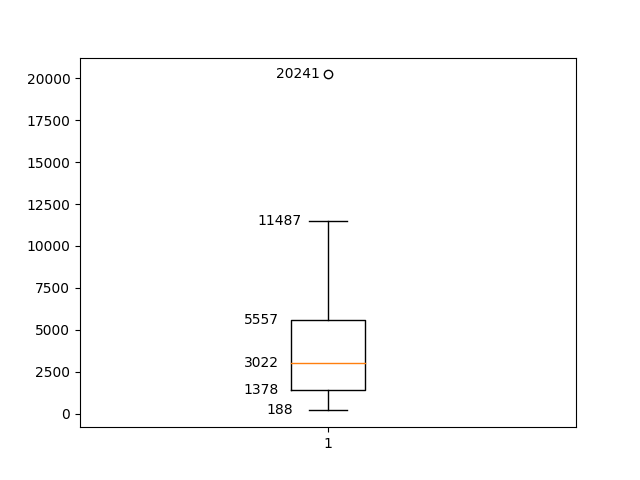
\includegraphics[width=1 \linewidth]{figures/category_box.png}
	\caption{Boxplot over the size of the categories. Size meaning the amount of documents with the same category.}
	\label{fig:category_box}
\end{figure}

\subsection{Taxonomy}
The taxonomy field describes a hierarchical structure of the topical or geographical subject of the articles.
This field is only partially observed within the dataset, which means that roughly $50\%$ of the articles contain this field.
Each article can also contain multiple taxonomies.
We observe some general patterns when traversing this field, which are:
\begin{itemize}
	\item PLACES/Country/Region/Town
	\item TOPICS/Sub-Topic/Subsub-topic
\end{itemize}
Examples of this field are:
\begin{itemize}
	\item PLACES/Danmark/Nordjylland/Aalborg/Lillevorde
	\item TOPICS/Religion/Christianity
\end{itemize}
About $80\%$ of the observed fields contain the 'PLACES' variable and $20\%$ use the 'TOPICS' variable. 
